%!TEX root = ../agi_mfwis415af4l.tex
\section{Projektplanung}
\label{concept}

\subsection{Pflichtenheft}\\
\\
\textbf{Allgemeines}
\\Dieses Pflichtenheft beschreibt die Anforderungen für die Erstellung einer mobilen Applikation zur Verwaltung der Kalorienzunahme und die Bereitstellung von statistischen Übersichten von einem gewählten Zeitraum.\\
\textbf{Ziele der Aufgabenstellung}\\
Food4Life möchte mit der Applikation eine Kalorientracker-App in Form eines Tagebuchs ermöglichen. Verschiedene Übersichten über Monate, Tage etc. bieten eine simple und angenehme Oberfläche, zur Verwaltung und Verwendung der einzelnen Lebensmittel und Menüs.\\
\textbf{Zielgruppe}\\
Die Zielgruppe der Applikation sind Menschen, die ihre Kalorien verwalten wollen.\\
\textbf{Systemvorrausetzungen}\\
Für die Benutzung der App ist ein Smartphone oder Tablet mit einer Android Version 4.0 oder höher erforderlich. Ein Internetzugang ist nicht erforderlich.\\
\textbf{Beschreibung der Anforderungen}\\
Die Benutzer der App sollen folgende Funktionen haben:
\begin{itemize}
\item Kalorientageshöchstwert festlegen und verändern
\item 	Anzeige der Summe der konsumierten Kalorien an einem Tag und des Kalorientageshöchstwert
\item 	Anzeige der durchschnittlichen konsumierten Kalorien der letzten 7, 14 und 30 Tage
\item 	Anzeige aller Einträge des Tagebuches zeitlich aufsteigend sortiert und tageweise untergliedert
\item 	Beliebige Navigation durch den Kalender
\item 	Navigation zum aktuellen Tag im Kalender
\item 	Hinzufügen, Bearbeiten, Kopieren, Verschieben und Löschen eines Eintrags
\item 	Anlegen, Bearbeiten und Löschen von benutzerdefinierten Menüs
\item 	Hinzufügen, Bearbeiten und Löschen eines Lebensmittels
\item 	Hinzufügen und Löschen einer Einheit\\
\end{itemize}


\subsection{Projektablaufplan}

\subsection{Planung der Software}

\subsubsection{Planung der Mockups}\\

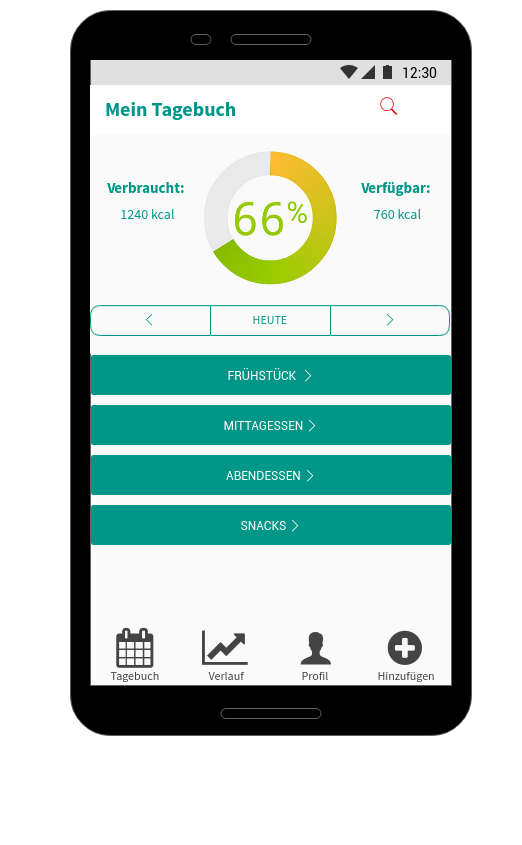
\includegraphics[scale=0.3]{img/mockup.png}\\

Die Startseite der App soll das Herzstück der App darstellen. Beim Öffnen der App soll dem User übersichtlich vermittelt werden, wie viele Kalorien Er/Sie zu sich genommen hat und wie viele Kalorien vom individuellen Tagesbedarf noch zur Verfügung stehen. Zusätzlich soll der Verbrauch der Kalorien visuell mithilfe einer Fortschrittsanzeige (Progress Bar) dargestellt werden. Des Weiteren wird auf der Startseite immer das tagesaktuelle Datum angezeigt. Mithilfe von vier Buttons, soll es dem User möglich sein, die zu sich genommen Lebensmittel einzutragen und kategorisch nach Tageszeit bzw. Mahlzeit zu gliedern. Über die Startseite soll der User zu den weiteren Seiten innerhalb App gelangen, wobei hierfür mehrere Buttons am Ende des Bildschirmes zur Verfügung stehen. So gelangt der User beispielsweise per Klick zu seinem persönlichen Tagebuch mit Kalenderübersicht oder kann über den Button "Profil" persönliche Daten zu Name, Gewicht, Größe und Kalorientagesbedarf hinterlegen.


\subsubsection{Planung der Datenstrukturen und Schnittstellen}

\subsubsection{Planung der Activities und Layouts}

\subsubsection{Planung der Navigation und des Datenaustausches zwischen den Activities }

\subsection{Geplante Aufgabenverteilung im Team}\\

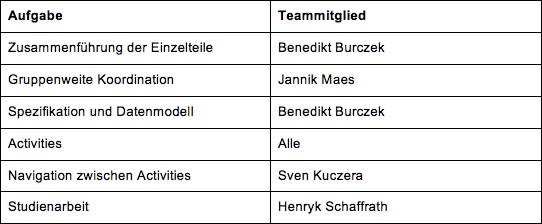
\includegraphics[scale=0.8]{img/geplanteAugabenVerteilung}\\
